\chapter{Theory of machine learning}
\label{chap:ml}

Machine learning provides a framework for constructing functions that map inputs to outputs by optimising a parametric model against labelled examples.  In high-energy physics the canonical task is classification: given a set of measured quantities describing an event, assign it to one of $K$ classes.  The theoretical tools introduced in this chapter, multi-layer perceptrons, recurrent networks and transformers, address this task with increasing architectural complexity.

\section{Multi-layer perceptron}

A multi-layer perceptron (MLP) is a directed acyclic graph of parametric transformations organised into $L$ sequential layers.  Each layer $\ell$ maps an input vector $\mathbf{h}^{(\ell-1)}\in\mathbb{R}^{n_{\ell-1}}$ to an output $\mathbf{h}^{(\ell)}\in\mathbb{R}^{n_{\ell}}$ by an affine transformation followed by a pointwise nonlinearity $\sigma$,
\begin{equation}
\mathbf{h}^{(\ell)} = \sigma\!\left(W^{(\ell)}\mathbf{h}^{(\ell-1)} + \mathbf{b}^{(\ell)}\right), \qquad W^{(\ell)}\in\mathbb{R}^{n_{\ell}\times n_{\ell-1}},\quad \mathbf{b}^{(\ell)}\in\mathbb{R}^{n_{\ell}}.
\end{equation}
The input is $\mathbf{h}^{(0)}=\mathbf{x}$ and the final layer produces the network output $\hat{\mathbf{y}}=\mathbf{h}^{(L)}$.  The parameters $\theta=\{W^{(\ell)},\mathbf{b}^{(\ell)}\}_{\ell=1}^{L}$ are learned by minimising a loss functional over a training dataset.

A common nonlinearity for hidden layers is the rectified linear unit,
\begin{equation}
\mathrm{ReLU}(z) = \max(0,z),
\end{equation}
which preserves positive activations unchanged and maps negative ones to zero.  Its piecewise-linear form avoids the vanishing-gradient problem that afflicts saturating activations such as $\tanh$, while remaining a universal approximator when composed across multiple layers \cite{Hornik_Universal_1989}.
\subsection{Input normalisation}
\label{sec:normalisation}

Before training, input features are standardised to zero mean and unit variance across the training set.  For each feature $x_j$ with empirical mean $\mu_j$ and standard deviation $\sigma_j$, the standardised value is
\begin{equation}
\tilde{x}_{j} = \frac{x_{j} - \mu_{j}}{\sigma_{j}}.
\end{equation}
Standardisation ensures that features with different physical scales contribute equally to the gradient updates and prevents large-magnitude inputs from dominating the loss landscape.
\subsection{Binary classification}
\label{sec:binary}

In binary classification the network produces a single output score $\hat{y}\in(0,1)$ interpreted as the probability $P(y=1\mid\mathbf{x})$ that the input belongs to the positive class.  This is achieved by taking the final layer to have a single unit with the sigmoid activation
\begin{equation}
\sigma(z) = \frac{1}{1+e^{-z}},
\end{equation}
which squashes any real-valued pre-activation $z$ into the unit interval.  The corresponding loss functional is the binary cross-entropy,
\begin{equation}
\mathcal{L}_{\mathrm{BCE}} = -\frac{1}{N}\sum_{i=1}^{N} \Bigl[ y_{i}\log\hat{y}_{i} + (1-y_{i})\log(1-\hat{y}_{i}) \Bigr],
\label{eq:bce}
\end{equation}

where $y_i\in\{0,1\}$ is the true label and $\hat{y}_i$ the predicted probability for the $i$-th example.  The loss is a proper scoring rule: it is minimised if and only if $\hat{y}_i = P(y=1\mid\mathbf{x}_i)$, so gradient descent on $\mathcal{L}_{\mathrm{BCE}}$ pushes the network toward the true posterior.

\subsection{Multi-class classification}
\label{sec:multiclass}

When the target space has $K>2$ mutually exclusive classes, the output layer is extended to $K$ units with the softmax activation
\begin{equation}
\hat{y}_{k} = \frac{e^{z_{k}}}{\sum_{j=1}^{K}e^{z_{j}}}, \qquad k=1,\dots,K,
\label{eq:softmax}
\end{equation}
where $z_k$ are the pre-activations of the final layer.  By construction $\hat{y}_k\in(0,1)$ and $\sum_k\hat{y}_k=1$, so the output vector forms a valid discrete probability distribution over the $K$ classes.  The softmax is the multi-class generalisation of the sigmoid: for $K=2$ it reduces to equation \eqref{eq:bce} up to reparametrisation.  The corresponding loss is the categorical cross-entropy,
\begin{equation}
\mathcal{L}_{\mathrm{CCE}} = -\frac{1}{N}\sum_{i=1}^{N}\sum_{k=1}^{K} y_{ik}\log\hat{y}_{ik},
\label{eq:cce}
\end{equation}
where $y_{ik}\in\{0,1\}$ is the one-hot encoded true label ($y_{ik}=1$ if example $i$ belongs to class $k$, zero otherwise).  Only the term corresponding to the true class contributes to the sum for each example, so minimising $\mathcal{L}_{\mathrm{CCE}}$ drives the network to concentrate probability mass on the correct class.

In the context of aQGC searches, the multi-class formulation is particularly natural.  Each operator family, or individual operator within a family, defines a distinct signal class and the softmax output $\hat{y}_k$ provides a per-event estimate of the posterior probability for operator $k$.  A single multi-class network can therefore simultaneously discriminate among all operator types, replacing the combination of multiple binary classifiers that would otherwise be required.

Parameters are updated by stochastic gradient descent.  At each step a mini-batch $\mathcal{B}\subset\{1,\dots,N\}$ is drawn and the parameter vector updated as
\begin{equation}
\theta \leftarrow \theta - \eta\,\nabla_{\theta}\, \frac{1}{|\mathcal{B}|}\sum_{i\in\mathcal{B}}\ell(\hat{y}_i,y_i),
\end{equation}
where $\eta$ is the learning rate and $\ell$ is the per-example loss from either \eqref{eq:bce} or \eqref{eq:cce}.  The gradients are computed efficiently by backpropagation, which applies the chain rule layer by layer from the output back to the input \cite{Rumelhart_Backprop_1986}.



\section{Recurrent neural network}

A recurrent neural network processes sequential inputs $(\mathbf{x}_1,\mathbf{x}_2,\dots,\mathbf{x}_T)$ of variable length $T$ by maintaining a hidden state that is updated at each step and carries information forward through the sequence.  Vanilla recurrent architectures suffer from vanishing and exploding gradients when $T$ is large, because backpropagation through time involves repeated multiplication by the same weight matrix, causing gradient norms to shrink or grow exponentially with depth.  The long short-term memory (LSTM) \cite{Hochreiter_LSTM_1997} resolves this by introducing a dedicated cell state $\mathbf{c}_t\in\mathbb{R}^{d}$ that carries long-range information along an additive path, insulated from the multiplicative degradation that affects the hidden state $\mathbf{h}_t\in\mathbb{R}^{d}$.

At each step $t$ the LSTM computes three gating vectors from the concatenation of the previous hidden state $\mathbf{h}_{t-1}$ and the current input $\mathbf{x}_t$,
\begin{align}
\mathbf{f}_{t} &= \sigma\!\left(W_{f}\,[\mathbf{h}_{t-1},\mathbf{x}_{t}]+\mathbf{b}_{f}\right), &&\text{(forget gate)}\\[3pt]
\mathbf{i}_{t} &= \sigma\!\left(W_{i}\,[\mathbf{h}_{t-1},\mathbf{x}_{t}]+\mathbf{b}_{i}\right), &&\text{(input gate)}\\[3pt]
\mathbf{o}_{t} &= \sigma\!\left(W_{o}\,[\mathbf{h}_{t-1},\mathbf{x}_{t}]+\mathbf{b}_{o}\right), &&\text{(output gate)}
\end{align}
where $\sigma$ is the sigmoid activation and $[\cdot,\cdot]$ denotes concatenation.  Each gate is a vector in $(0,1)^d$ whose entries act as soft switches.  A candidate update to the cell state is computed as
\begin{equation}
\tilde{\mathbf{c}}_{t} = \tanh\!\left(W_{c}\,[\mathbf{h}_{t-1},\mathbf{x}_{t}]+\mathbf{b}_{c}\right).
\end{equation}
The cell state and hidden state are then updated by
\begin{align}
\mathbf{c}_{t} &= \mathbf{f}_{t}\odot\mathbf{c}_{t-1} + \mathbf{i}_{t}\odot\tilde{\mathbf{c}}_{t}, \label{eq:lstm_cell}\\[3pt]
\mathbf{h}_{t} &= \mathbf{o}_{t}\odot\tanh(\mathbf{c}_{t}), \label{eq:lstm_hidden}
\end{align}
where $\odot$ denotes elementwise multiplication.  The forget gate $\mathbf{f}_t$ controls what fraction of the previous cell state is retained, when its entries are close to one the cell state is preserved unchanged across the step, allowing gradients to flow back through equation \eqref{eq:lstm_cell} without attenuation.  The input gate $\mathbf{i}_t$ controls how much of the candidate update $\tilde{\mathbf{c}}_t$ is written into the cell state and the output gate $\mathbf{o}_t$ determines what portion of the updated cell state is exposed as the hidden state.  The gating structure is illustrated in Figure~\ref{fig:lstm_cell}.

\begin{figure}[htbp]
  \centering
  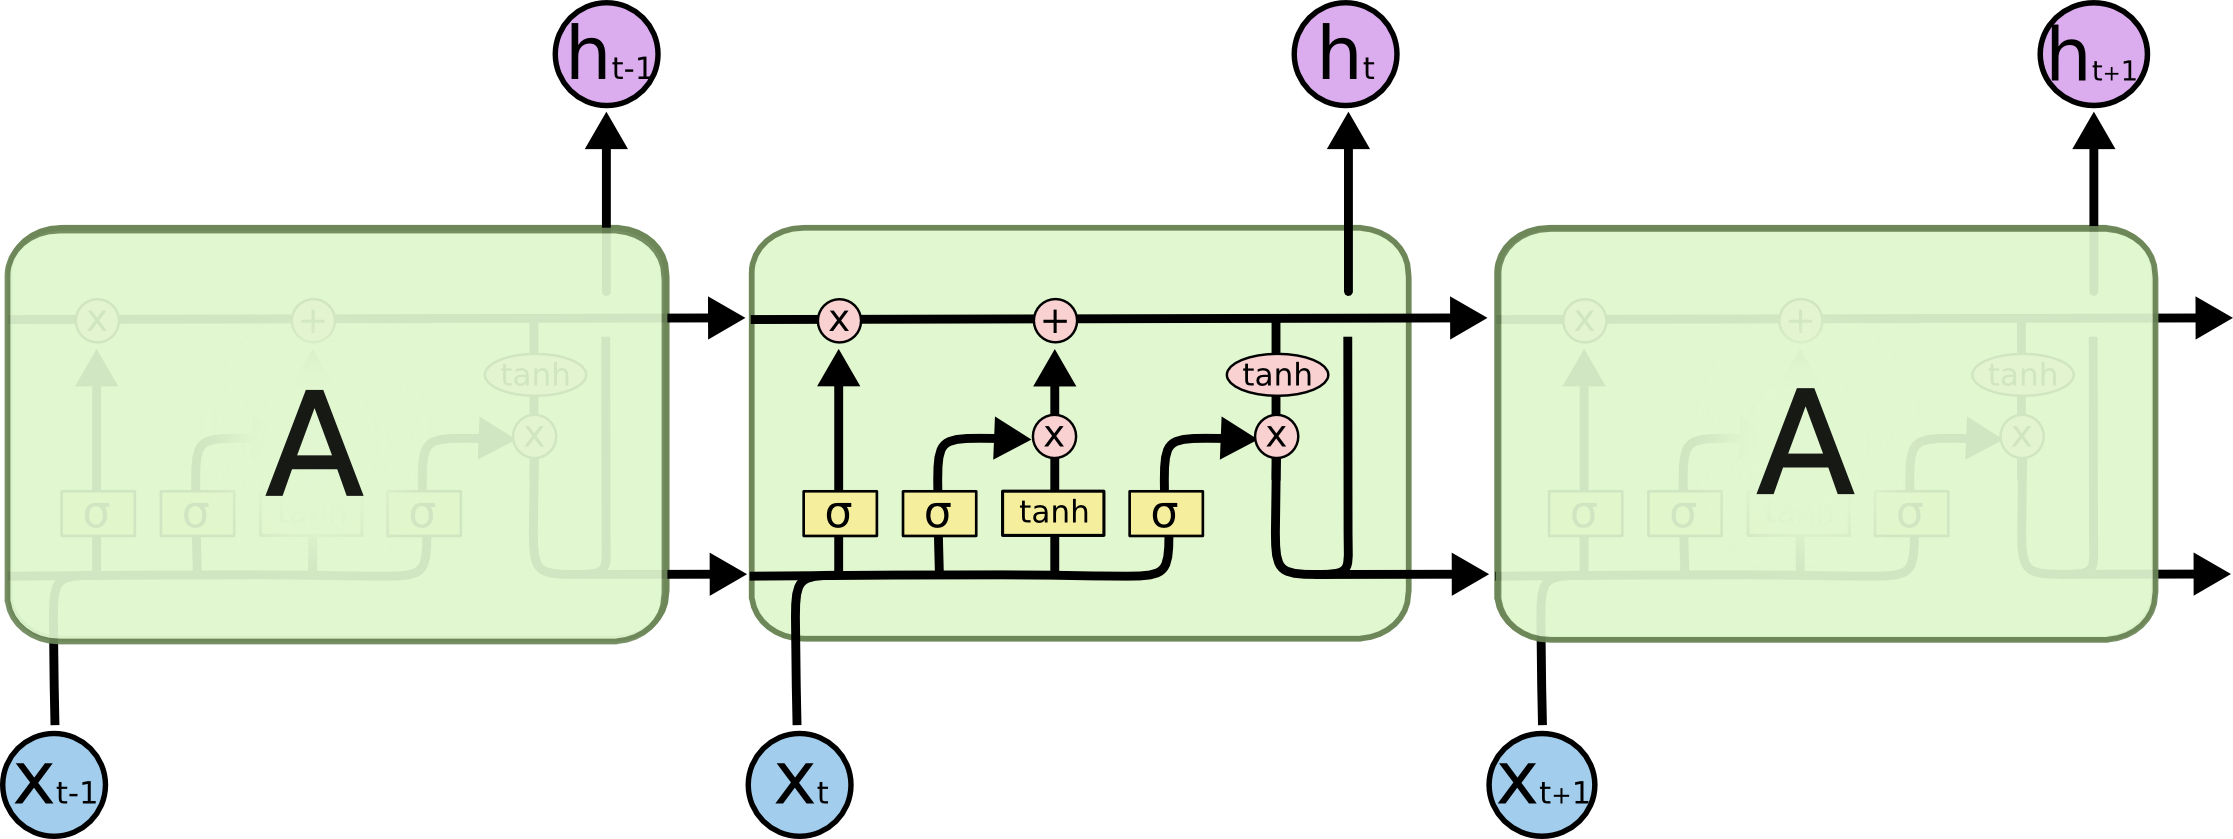
\includegraphics[width=0.65\textwidth]{figures/LSTMcell.png}
  \caption{LSTM cell showing three consecutive time steps.  The expanded cell shows the internal gating structure: the forget gate, input gate, candidate cell update and output gate each receive the concatenation of the previous hidden state $\mathbf{h}_{t-1}$ and the current input $\mathbf{x}_t$.  The cell state $\mathbf{c}_t$ flows along the horizontal additive path (upper horizontal line), enabling long-range gradient propagation, the hidden state $\mathbf{h}_t$ is derived from it via the output gate and a $\tanh$ squashing, as described by equations~\eqref{eq:lstm_cell} and~\eqref{eq:lstm_hidden}. ~\cite{Olah_LSTM_2015}.}
  \label{fig:lstm_cell}
\end{figure}

After processing all $T$ steps, the final hidden state $\mathbf{h}_T$ encodes a summary of the entire input sequence.  A classification head applied to $\mathbf{h}_T$ produces the output probabilities via sigmoid for binary classification or softmax for the multi-class case, as described in sections \ref{sec:binary} and \ref{sec:multiclass}.  All weight matrices $\{W_f, W_i, W_o, W_c\}$ and bias vectors $\{b_f, b_i, b_o, b_c\}$ are shared across all $T$ steps, so the same learned function is applied regardless of sequence length, making the LSTM naturally suited to inputs such as collections of reconstructed particles or jets where the multiplicity varies event by event.

\section{Transformer architecture}

The transformer \cite{Vaswani_Attention_2017} abandons recurrent processing in favour of a fully parallel architecture built around the scaled dot-product attention mechanism.  Given a sequence of $T$ input vectors assembled as rows of a matrix $X\in\mathbb{R}^{T\times d}$, three linear projections produce queries, keys and values,
\begin{equation}
Q = XW^{Q},\quad K = XW^{K},\quad V = XW^{V}, \qquad W^{Q},W^{K},W^{V}\in\mathbb{R}^{d\times d_k}.
\end{equation}
The attention output is
\begin{equation}
\mathrm{Attention}(Q,K,V) = \mathrm{softmax}\!\left(\frac{QK^{\top}}{\sqrt{d_{k}}}\right)V,
\label{eq:attention}
\end{equation}
where the $\sqrt{d_k}$ factor prevents the dot products from entering the saturated region of the softmax for large $d_k$.  The $(i,j)$ entry of the softmax argument is the inner product $Q_i\cdot K_j/\sqrt{d_k}$, measuring how relevant position $j$ is to position $i$.  The output at position $i$ is therefore a weighted average of all value vectors, with weights given by these relevance scores.

In practice $H$ independent attention heads are computed in parallel on lower-dimensional projections and their outputs concatenated,
\begin{equation}
\begin{aligned}
\mathrm{MultiHead}(Q,K,V) &= \mathrm{Concat}(\mathrm{head}_1,\dots,\mathrm{head}_H)\,W^{O}, \\
\mathrm{head}_h &= \mathrm{Attention}(QW_h^Q,\,KW_h^K,\,VW_h^V).
\end{aligned}
\end{equation}
Each head can attend to different structural features of the sequence simultaneously.  The attention block is followed by a position-wise feedforward network applied identically at each position, together forming a transformer encoder layer.  Residual connections and layer normalisation \cite{Ba_LayerNorm_2016} stabilise training.

The key distinction from recurrent architectures is that equation \eqref{eq:attention} computes interactions between every pair of positions $(i,j)$ in a single matrix operation, with no sequential dependency.  The computational cost of the attention step scales as $\mathcal{O}(T^{2}d_{k})$, so the architecture is most advantageous when $T$ is large enough that the rich pairwise interaction structure justifies this cost.  In particle physics applications, where a jet or event can be represented as a sequence of $\mathcal{O}(10^2)$ or more constituent particles or detector objects, the transformer's ability to capture long-range correlations across the full sequence in a single layer gives it a structural advantage over recurrent models that propagate information step by step and may lose distant context.  A classification token appended to the sequence, or a pooling operation over the final hidden states, extracts a fixed-length representation to which a sigmoid or softmax head is applied.

\section{Permutation importance}
\label{sec:permutation_importance}

Once a network is trained it is often necessary to quantify how much each input feature contributes to its predictions, both as a cross-check that the model relies on the variables expected to be discriminating and to identify redundant inputs that could be dropped. A simple, model-agnostic way to do this is \emph{permutation importance}, which probes how strongly a trained model depends on each feature without retraining it.

Let $f$ denote the trained model and let $A_0$ be a scalar performance metric evaluated on a labelled evaluation sample $\mathcal{D}=\{(\mathbf{x}_i,y_i)\}_{i=1}^{N}$, such as the classification accuracy or the area under the ROC curve. For a given input feature $j$, a perturbed sample $\mathcal{D}^{\pi_j}$ is built by randomly permuting the values of that feature across the $N$ evaluation events,
\begin{equation}
  x^{(j)}_i \;\longrightarrow\; x^{(j)}_{\pi(i)},
  \qquad \pi\ \text{a random permutation of}\ \{1,\dots,N\},
\end{equation}
while every other feature and the labels are left untouched. The permutation destroys any association between feature $j$ and the label but leaves its marginal distribution intact, so the model is evaluated on inputs that remain individually realistic but in which feature $j$ has been rendered uninformative. Re-evaluating the frozen model on $\mathcal{D}^{\pi_j}$ yields a degraded metric $A_j$, and the importance of the feature is the resulting drop
\begin{equation}
  \Delta A_j \;=\; A_0 - A_j \;\ge\; 0,
\end{equation}
which is large for a feature the decision boundary depends on and consistent with zero for one the model ignores. To compare features on a common scale the drops are normalised to unit sum,
\begin{equation}
  I_j \;=\; \frac{\Delta A_j}{\sum_{k}\Delta A_k},
  \label{eq:rel_importance}
\end{equation}
and $I_j$ is referred to as the relative feature importance.

Two properties of the method matter for the interpretation of the resulting rankings. First, because the model is never retrained, $I_j$ measures the reliance of that particular trained model on feature $j$ rather than the intrinsic separating power of the variable: a feature that is informative but whose information is also carried by a correlated partner can be permuted with little metric loss, and is then assigned a low importance. Permutation importance therefore tends to share, and partly mask, the importance of correlated inputs. Second, the procedure is stochastic through the choice of permutation $\pi$; in practice it is repeated over several permutations and the resulting importances averaged, so that the residual scatter is small compared with the differences between features.